% !TEX root = ../Thesis.tex
\chapter{Evaluation}

In this section we want to talk about the evaluation as a whole. We want to look at the phrases we took, how we carried it out, the results observed and shortly discuss what all of this means.

\section{MacKenzie Phrase Set}
One precondition for the evaluation is to use the MacKenzie Phrase Set\footnote{http://www.yorku.ca/mack/PhraseSets.zip}. Basically, this is just a set of 500 phrases. According to the paper \cite{10.1145/765891.765971}, such a phrase set should use phrases of moderate length, that are easy to remember and representative for the target language. These phrases do not contain any punctuation. Some of them use uppercase characters, but the authors mention, that participants can also be instructed to ignore the case of the characters. 
%The complete MacKenzie Phrase can be downloaded at \hyperlink{http://www.yorku.ca/mack/PhraseSets.zip}{http://www.yorku.ca/mack/PhraseSets.zip}.
\\
Some statistics for the whole phrase set, also found in the original paper \cite{10.1145/765891.765971}: The MacKenzie phrase set consists of 500 phrases, that have a minimum length of 16, a maximum length of 43 and an average length of 28.61 characters. On the whole, 2712 words were used, which consist of 1163 unique words. A phrase consists of a minimum of 1, a maximum of 13 and on average of 4.46 words.

\section{Task of the Participants}
The task of the participants is to copy 15 "random" phrases. They are not really random, but adjacent phrases from the downloadable MacKenzie Phrase Set (\url{http://www.yorku.ca/mack/PhraseSets.zip}{http://www.yorku.ca/mack/PhraseSets.zip}). As they are not in a specific order, e.g. alphabetic order, we decide to do it like this.\\
TODO: PICTURE OF EVALUATION SCENE.
The participants see two text fields. On the top is the phrase to copy, on the bottom the words/phrase they write. If the given phrase matches the user inputted phrase, a sound sounds, such that the participants know when they finish one specific phrase. After that, a new phrase appears until 15 phrases are correctly inputted. If an incorrect word is entered, the user either can use the word suggestions (fig \ref{fig:write_suggestions}) or delete the wrong word and try to write it again. If a mistake is only noticed later on, the participants have to remove all words and characters up to and including the wrong word by using the backspace button.\\
After this first step, in the second step, we shortly explain two functions of the keyboard, which they can test afterwards. First the scaling buttons and then the function to add a new word. This is important, because we want to know if they find these functions useful and well implemented.\\
The last step of the evaluation is to fill a questionnaire. First it has some general questions about the participant's experience in VR. Then there is a block of questions in the form of a system usability scale. Per question, there are five possibilities to set the cross. From 1 (strongly disagree) to 5 (strongly agree). The questions are structured in such a way, that if the user is highly satisfied with everything, they would alternately make a cross at the 5 and 1. TODO: FRAGEBOGEN ALS ANHANG BEIFÜGEN.

\section{Carry-out}
To carry out the evaluation, we used two different VR systems. One was a setup with a HTC vive and HTC vive controllers. The other one included an Oculus Rift headset with corresponding controllers. Even though these are two different systems, it does not change much for the participants. In fact, only the controllers and their buttons differ a bit.\\
To find participants, we wrote an email to students from our university, and asked family members and friends. All in all, eleven people got in touch with us and participated at our evaluation. Every participant got the same explanation to give everybody the same foundation of knowledge.\\
We told them that if they are close enough to the keyboard, then the color gets a bit brighter, and they are in the keyboard's hitbox. We said, the keyboard is movable, if they press and hold the controller's grip button in the hitbox of the keyboard. If they release it, the keyboard gets static again and stays where it got put.\\
To write, they do also have to be in the hitbox of the keyboard but not pressing and holding the grip button, but the trigger button. Then they had to make a gesture over the characters of the keyboard to write a word. We also told them, that if they do a full gesture and a word longer than one character is written, a space is automatically put behind the word. We also said to them, that single characters could be inputted by clicking on a key of the intended character. If they did so, no space is put, and they have to do it their own. In the English language, this is particularly important for the words "I" and "a".\\
We also told them, that if they made a gesture and a word was written, there may be one to four other choosable words. They could pick from them, if the word written in the text field is the wrong one. We especially mentioned the word ``the''. All the time ``thee'' would be written as the best match, therefore they would have to correct it every time.\\
They were also informed about the backspace. So, that if they use the backspace button after writing a word, the whole word gets deleted and afterwards only single characters get deleted.\\
We also told the participants, that we have enough time and that they should not hurry, but rather look, that the inputted words are correct. Because if they are not correct, they have to use the backspace a lot of times.

\section{Results}
Now, we want to talk about the results and some statistics.\\

\subsection{System Usability Scale}
First, we begin with the results of the SUS questions. These ten questions were:\\
1. I think that I would like to use this system frequently when I work in VR\\
2. I found the system unnecessarily complex\\
3. I thought the system was easy to use \\
4. I think that I need the support of a technical person to be able to use this system\\
5. I found the various functions in this system were well integrated\\
6. I thought there was too much inconsistency in this system\\
7. I would imagine that most people would learn to use this system very quickly\\
8. I found the system very cumbersome to use\\
9. I felt very confident using the system\\
10. I needed to learn a lot of things before I could get going with this system
\begin{table}[ht!]
    \centering
    \begin{tabular}{cccc} \toprule
        question&average score&perfect possible score&$\sigma$\\ \midrule
        1 & 4.27 & 5.0 & 0.445\\ 
        2 & 1.09 & 1.0 & 0.287\\
        3 & 4.64 & 5.0 & 0.481\\ 
        4 & 1.27 & 1.0 & 0.617\\
        5 & 4.64 & 5.0 & 0.481\\
        6 & 1.64 & 1.0 & 0.979\\
        7 & 4.64 & 5.0 & 0.481\\
        8 & 1.45 & 1.0 & 0.498\\
        9 & 4.09 & 5.0 & 0.514\\
        10 & 1.55 & 1.0 & 0.656\\
        \bottomrule
    \end{tabular}
    \caption{Results from the System Usability Scale (SUS) from the questionnaire (first ten questions)}
    \label{tab:table}
\end{table}

Question 9 got the worst score, but with it being a 4.09 out of 5, it is still pretty good. From these values, we can calculate a usability score. From the questions, whose perfect score is 5, we have to subtract 1 from the average score. And from the other questions we have to subtract their average score from 5. At the end, we have to sum up these values and multiply them by 2.5. Our calculated usability score is 88.18. This is a high score, and we are really satisfied with it.\\
We also have two other questions about the scale and add word functions:\\
11. The function to add words is well implemented and easy to use\\
12. The function to scale the keyboard is unnecessary\\
Question 11 got a score of 4.55 out of 5 and question 12 got a score of 2.18, whereby 1 would be ideal. We conclude from these two questions, that the ``add word function'' makes a good impression whereas the scale function does not perform so well.\\

\subsection{Writing Speed}
In the following table you can see how fast in average the participants were able to write their 15 phrases. We do also list the fastest and slowest value. Everything is measured in words per minute, which is calculated as follows:
\begin{equation}
    WPM = \frac{\mid T \mid}{S} \times 60 \times \frac{1}{5}
\end{equation}
where $T$ is all the phrases a participant had to write, hence $\mid T \mid$ is the number of characters a participant had to write. $S$ is the time in seconds they used to write all 15 phrases.\\
\begin{table}[ht!]
    \centering
    \begin{tabular}{cccc} \toprule
        participant&average WPM&lowest WPM&highest WPM\\ \midrule
        1 & 11.457 & - & -\\ 
        2 & 12.19 & - & -\\
        3 & 13.055 & - & -\\ 
        4 & 11.609 & 5.3 & 25.5\\
        5 & 12.578 & 6.83 & 21.65\\
        6 & 10.285 & 5.27 & 19\\
        7 & 12.423 & 6.1 & 24.41\\
        8 & 16.056 & 8.28 & 30.74\\
        9 & 13.363 & 7.96 & 24.15\\
        10 & 17.118 & 7.98 & 24.45\\
        11 & 10.067 & 4.71 & 14.55\\
        \bottomrule
        average&12.75&6.55&23.06\\
        \bottomrule
    \end{tabular}
    \caption{average WPM, lowest WPM and highest WPM per participant. For the first three, we failed to get this data.}
    \label{tab:WPM}
\end{table}
\clearpage

\begin{figure}
    \centering
    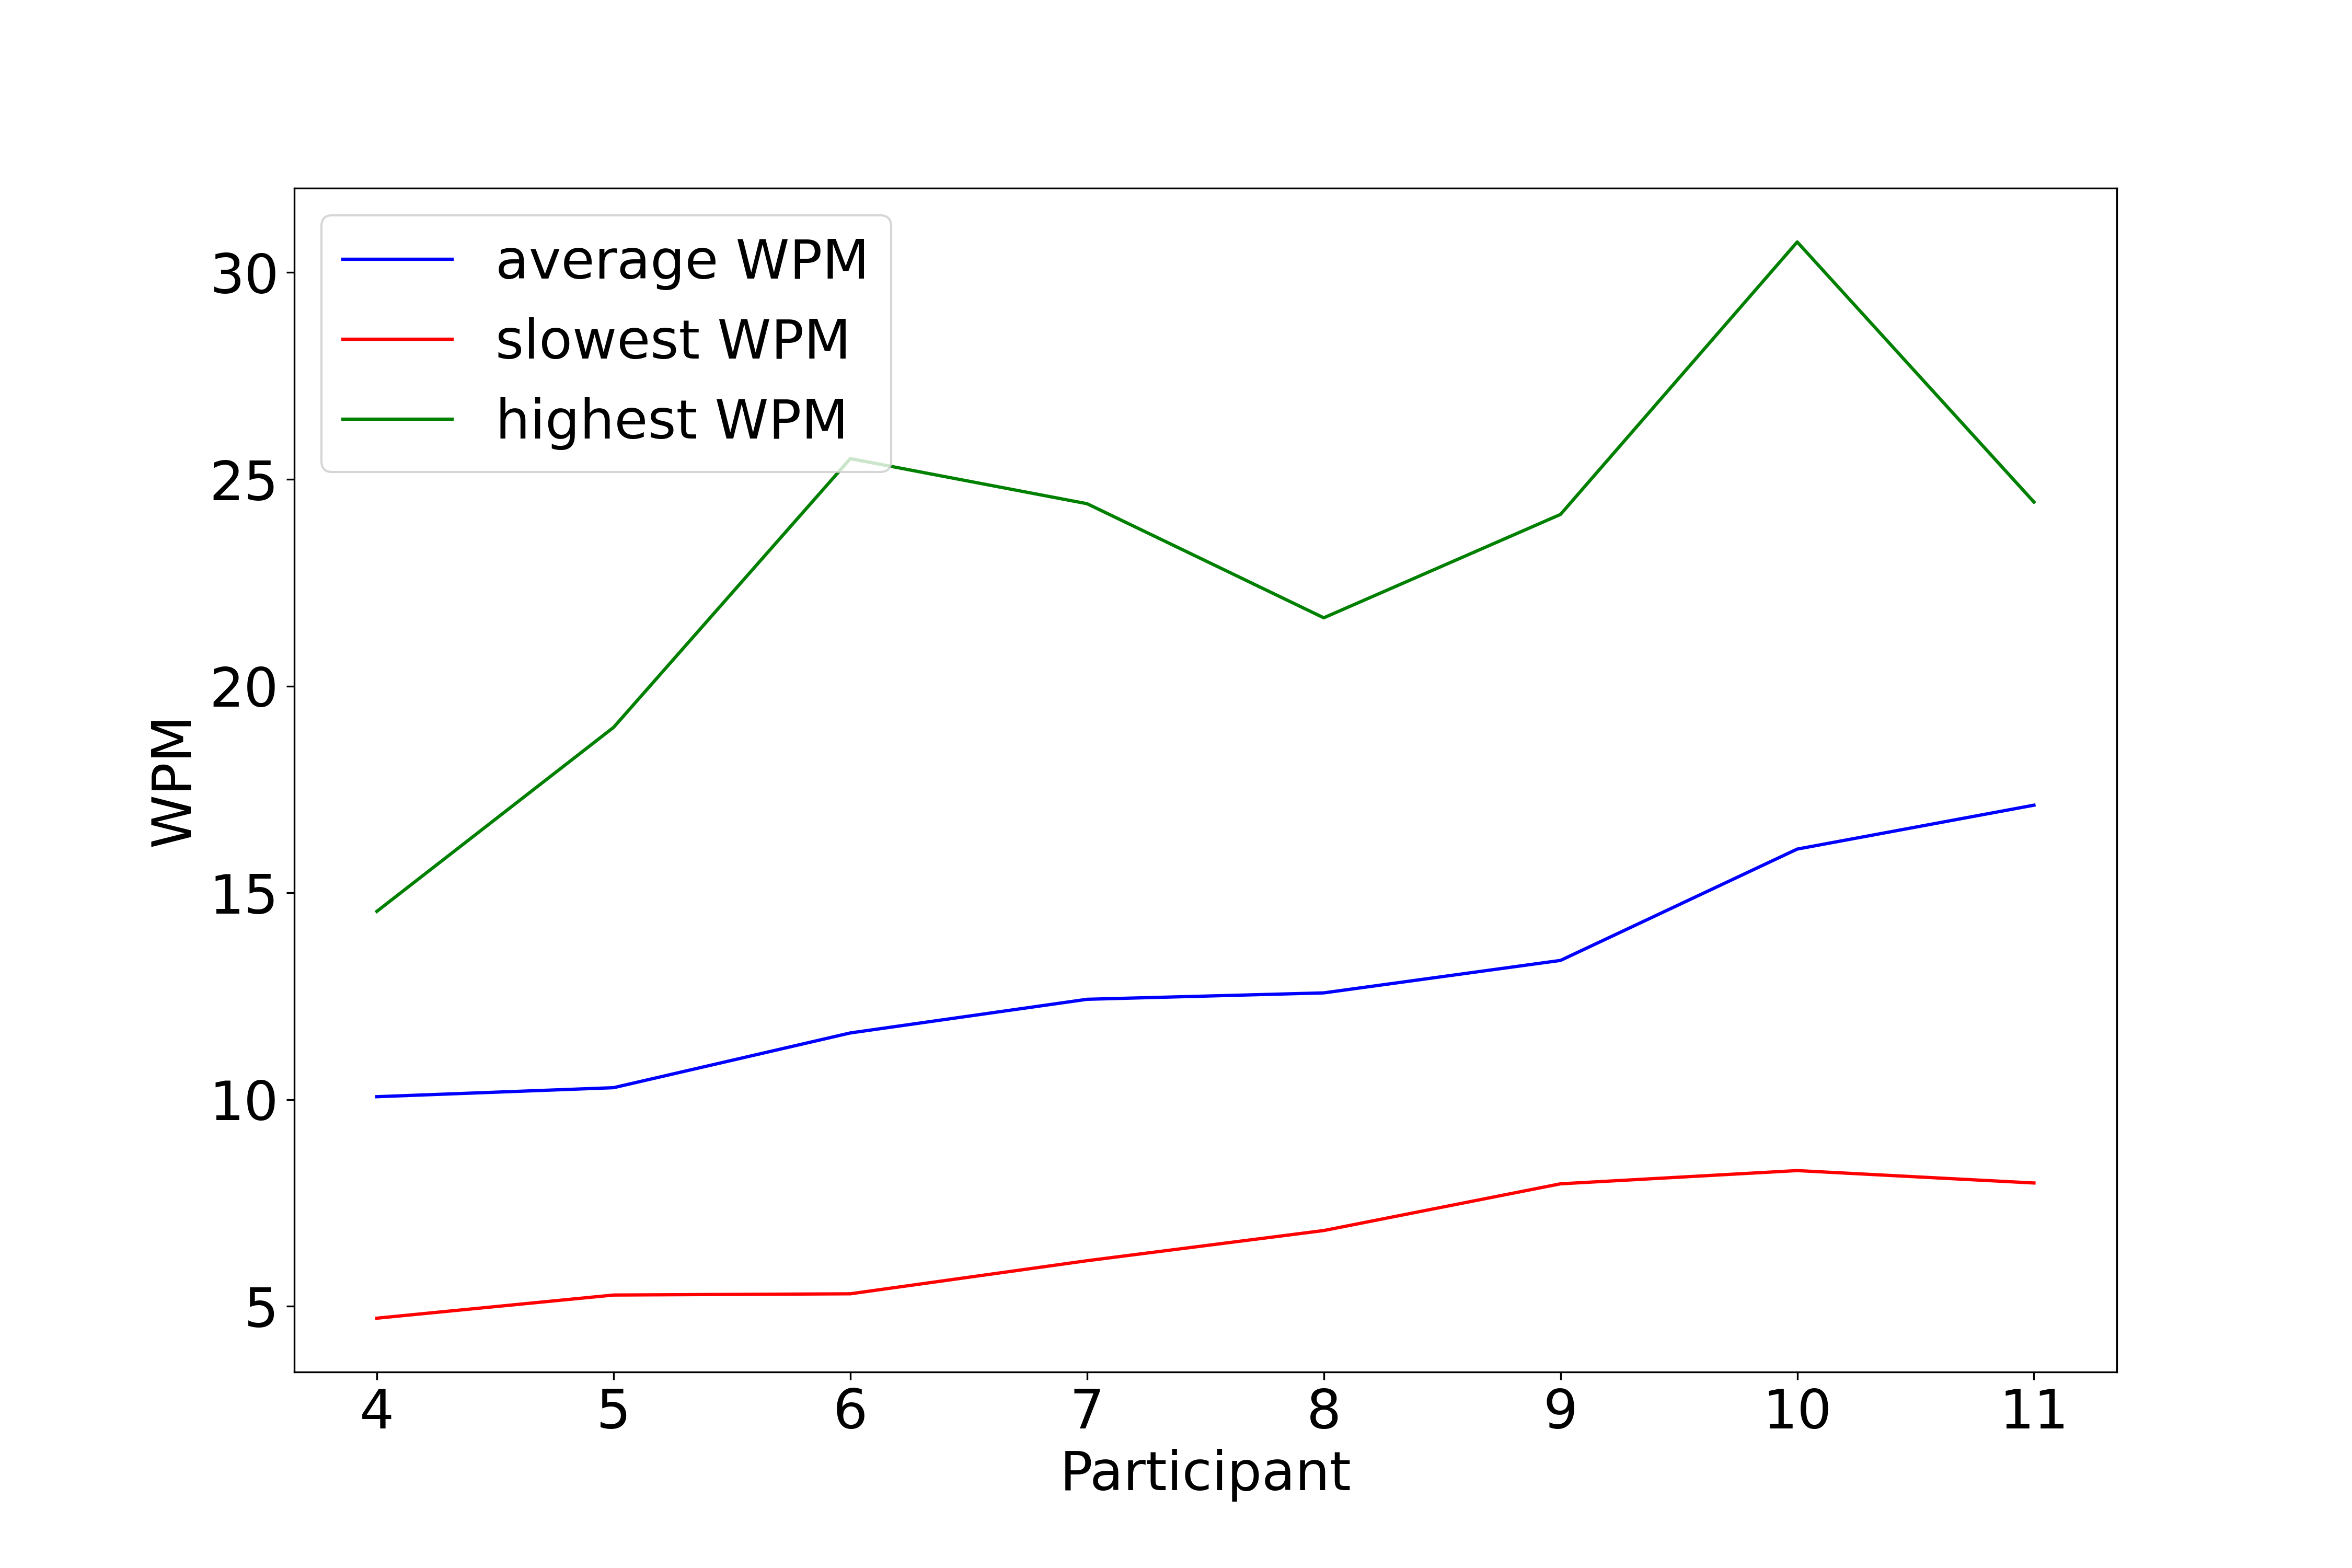
\includegraphics[width=0.8\textwidth]{WPM comparison.png}
    \caption{average WPM, lowest WPM and fastest WPM per participant 4-11}
    \label{fig:WPM}
\end{figure}
As we can see in fig \ref{fig:WPM}, the faster the participant is in average, most of the time they do also have higher lowest and highest WPM values. The lowest WPM values mostly come about because a participant made a mistake and had to delete a lot and basically write the phrase two times. On the other hand, the highest WPM values come about because a participant made no mistake in writing the phrase. \\

Next, we want to look at the WPM values of the users and their experience on one hand in VR writing and on the other hand in word-gesture keyboards:\\
\begin{figure}
    \centering
    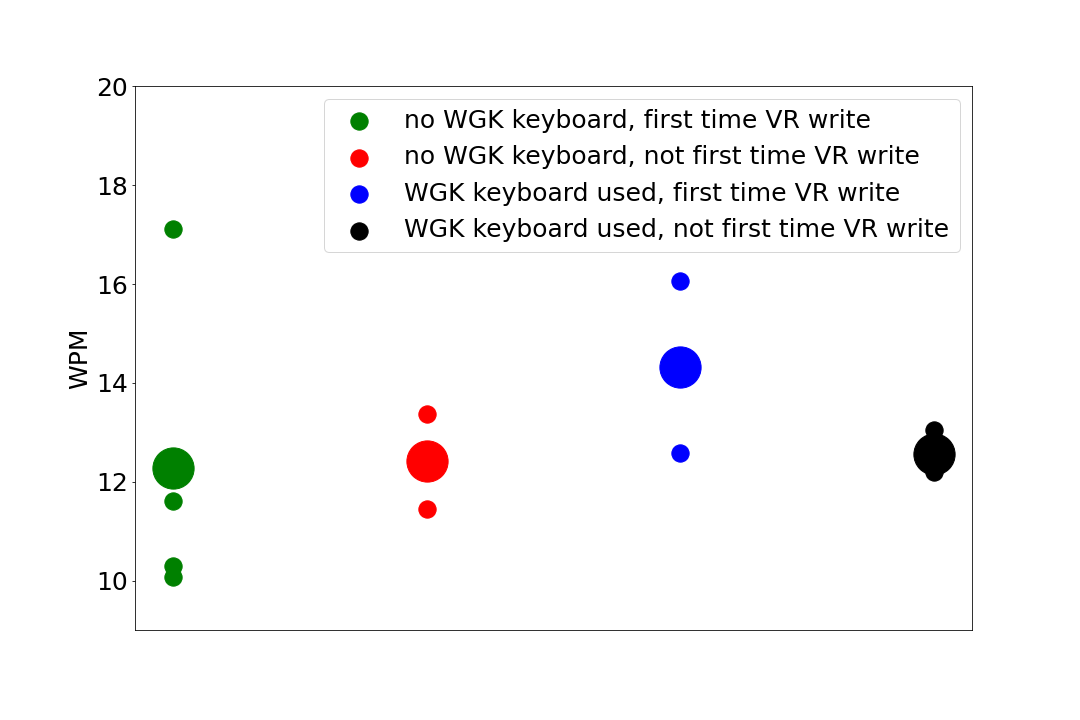
\includegraphics[width=0.8\textwidth]{Comparison_yesno.png}
    \caption{Average WPM per group of participant, grouped by their experience in VR writing and word-gesture keyboards}
    \label{fig:WPM_yesno}
\end{figure}
\\

CALCULATE KEYBOARD AND USER ERROR RATE (\#WRONG CHARACTERS OF WORDS NOT FOUND VS NOT CORRECTED)

\section{Discussion}